\documentclass[aspectratio=169,11pt]{beamer}

% ============================================================
% PACKAGES
% ============================================================
\usepackage{graphicx}
\usepackage{tikz}
\usetikzlibrary{positioning,arrows.meta}
\usepackage{xcolor}
\usepackage{booktabs}
\usepackage{tabularx}
\usepackage{array}
\usepackage{ragged2e}
\usepackage{hyperref}

% ============================================================
% COLORS - SAME AS PHASE-I
% ============================================================
\definecolor{GEUBlue}{RGB}{20,55,105}
\definecolor{GEULightBlue}{RGB}{238,244,251}
\definecolor{GEUGrey}{RGB}{90,90,90}
\definecolor{GEULightGrey}{RGB}{245,246,248}

% ============================================================
% BEAMER SETTINGS
% ============================================================
\usetheme{default}
\setbeamertemplate{navigation symbols}{}
\setbeamertemplate{blocks}[rounded][shadow=false]

\setbeamercolor{normal text}{fg=black,bg=white}
\setbeamercolor{frametitle}{fg=GEUBlue}
\setbeamercolor{structure}{fg=GEUBlue}
\setbeamercolor{block title}{fg=GEUBlue,bg=GEULightBlue}
\setbeamercolor{block body}{fg=black,bg=GEULightBlue}

\setbeamerfont{frametitle}{size=\Large,series=\bfseries}

% ============================================================
% LOGO
% ============================================================
% Upload the Graphic Era logo with this filename to Overleaf.
\newcommand{\GEULogo}{graphicera_logo.png}

% ============================================================
% HEADER
% ============================================================
\setbeamertemplate{headline}{%
  \begin{tikzpicture}[remember picture,overlay]
    \node[
        anchor=north east,
        xshift=-0.30cm,
        yshift=-0.12cm
    ] at (current page.north east)
    {\includegraphics[height=0.62cm]{\GEULogo}};
  \end{tikzpicture}
  \vspace{0.72cm}
}

% ============================================================
% FRAME TITLE
% ============================================================
\setbeamertemplate{frametitle}{%
  \vspace{0.03cm}
  \insertframetitle\par
  \vspace{0.04cm}
  \textcolor{GEUBlue}{\rule{\textwidth}{0.9pt}}
  \vspace{0.03cm}
}

% ============================================================
% FOOTER
% ============================================================
\setbeamertemplate{footline}{%
  \leavevmode
  \hbox{%
  \begin{beamercolorbox}[
      wd=.82\paperwidth,
      ht=0.32cm,
      dp=0.10cm,
      leftskip=.3cm
  ]{author in head/foot}
    \tiny Department of Computer Science \& Engineering |
    Graphic Era (Deemed to be University)
  \end{beamercolorbox}%
  \begin{beamercolorbox}[
      wd=.18\paperwidth,
      ht=0.32cm,
      dp=0.10cm,
      rightskip=.3cm
  ]{date in head/foot}
    \hfill\tiny\insertframenumber/\inserttotalframenumber
  \end{beamercolorbox}}
}

% ============================================================
% CUSTOM COMMANDS
% ============================================================
\newcommand{\smallnote}[1]{%
\vspace{0.08cm}
{\scriptsize\color{GEUGrey}#1}
}

\newcommand{\placeholder}[1]{%
\textit{\color{GEUGrey}#1}
}

% ============================================================
% DOCUMENT INFORMATION
% ============================================================
\title{\textbf{Project-Based Learning}\\[2mm]\large Phase-II Evaluation}
\author{\textbf{Project Title}\\Team ID: XXXX}

\institute{
Department of Computer Science \& Engineering\\
Graphic Era (Deemed to be University), Dehradun
}

\date{Academic Session 2026--27}

% ============================================================
% DOCUMENT
% ============================================================
\begin{document}

% ============================================================
% SLIDE 1
% ============================================================
\begin{frame}[plain]

\begin{tikzpicture}[remember picture,overlay]

\draw[GEUBlue,line width=3pt]
(current page.north west) -- (current page.north east);

\node[
    anchor=north east,
    xshift=-0.45cm,
    yshift=-0.35cm
] at (current page.north east)
{\includegraphics[height=1.0cm]{\GEULogo}};

\node[
    align=center,
    text width=.84\paperwidth
] at ([yshift=.25cm]current page.center)
{
{\color{GEUBlue}
\fontsize{26}{30}\selectfont
\bfseries PROJECT-BASED LEARNING}
\\[3mm]

{\fontsize{18}{22}\selectfont
PHASE-II EVALUATION}
\\[7mm]

{\color{GEUGrey}
\Large\bfseries
\placeholder{TapNGo- A Bus Fare Verification And Payment System}}
\\[3mm]

{\color{GEUBlue}
\normalsize Team ID: DSCPP-III-2026-T078}
};

\node[
    align=center,
    anchor=south,
    yshift=.42cm
] at (current page.south)
{
\bfseries
Department of Computer Science \& Engineering\\
Graphic Era (Deemed to be University), Dehradun\\[-1mm]
\scriptsize Academic Session 2026--27
};

\end{tikzpicture}

\end{frame}

% ============================================================
% SLIDE 2
% ============================================================
\begin{frame}{Team \& Mentor Details}

\begin{columns}[T,totalwidth=\textwidth]

\column{.48\textwidth}

\begin{block}{Team Information}
\begin{tabular}{@{}ll@{}}
\textbf{Team ID:} & DSCPP-III-2026-T078\\
\textbf{Semester:} & 3rd\\
\textbf{Section:} & C, E, H, K\\
\textbf{Domain:} & \placeholder{CSE}
\end{tabular}
\end{block}

\column{.48\textwidth}

\begin{block}{Team Members}
1.\quad \placeholder{Karnika Jain -- 2510010541 (Team Lead)}\\
2.\quad \placeholder{Anirudh Bahuguna -- 2510013536}\\
3.\quad \placeholder{Aparajita Pant -- 2510011139}\\
4.\quad \placeholder{Aaditya Budakoti -- 2510290931}
\end{block}

\end{columns}

\vspace{2mm}

\begin{block}{Mentor}
\placeholder{Ms. Isha Deshmukh}
\hfill
\textbf{Interactions completed: 6}
\underline{\hspace{12mm}}
\end{block}

\vfill

% \smallnote{Brief Discussion: Introduce the team, project domain, mentor, and responsibilities of the team members.}

\end{frame}

% ============================================================
% SLIDE 3
% ============================================================
\begin{frame}{Phase-I Recap \& Feedback Incorporated}

\vspace{-5mm}

\begin{block}{Phase-I Status}
\placeholder{
Proposed TapNGo, a seat-level fare verification and payment system for buses, with a 3-state seat model and a driver status panel. Phase-I covered problem statement, objectives and requirement analysis.
}
\end{block}

\vspace{2mm}

\begin{columns}[T,totalwidth=\textwidth]

\column{.48\textwidth}

\textbf{\color{GEUBlue}Feedback Received}

\begin{itemize}\itemsep2pt
\item \placeholder{Define clearly how a seat moves between states}
\item \placeholder{Build a small working C++ prototype and test each part}
\item \placeholder{Maintain the project on GitHub with regular commits}
\end{itemize}

\column{.48\textwidth}

\textbf{\color{GEUBlue}Changes Incorporated}

\begin{itemize}\itemsep2pt
\item \placeholder{Fixed 3 seat states: Empty, Unverified, Verified}
\item \placeholder{Simple C++ program split into small modules}
\item \placeholder{GitHub repository created, one branch per member}
\end{itemize}

\end{columns}

\vfill

% \smallnote{ Brief Discussion: Explain the major feedback received during Phase-I and clearly demonstrate how it has been incorporated. }

\end{frame}

% ============================================================
% SLIDE 4
% ============================================================
\begin{frame}{Problem Statement \& Finalized Objectives}

\begin{block}{Problem Statement}
\placeholder{
On buses, paying the fare and getting a seat depends on a conductor, and checking every passenger’s ticket slows down boarding. TapNGo lets a passenger pay with a card at the seat, and shows the driver which seats are paid and which are not. The bus leaves only when every seat is verified.
}
\end{block}

\vspace{2mm}

\textbf{\color{GEUBlue}Finalized Objectives}

\begin{enumerate}\itemsep3pt
\item \placeholder{Develop a seat-level fare verification and card payment system}
\item \placeholder{Track every seat as Empty, Occupied Unverified or Occupied Verified}
\item \placeholder{Provide a real-time driver status panel (grey / red / green seat map)}
\item \placeholder{Allow departure only when no seat is unverified, reducing boarding delay}
\end{enumerate}

\vfill

% \smallnote{ Brief Discussion: Avoid repeating the complete Phase-I presentation. Focus on the finalized problem, scope and measurable objectives. }

\end{frame}

% ============================================================
% SLIDE 5
% ============================================================
\begin{frame}{Updated System Architecture / Workflow}

\vspace{-5mm}

\begin{center}

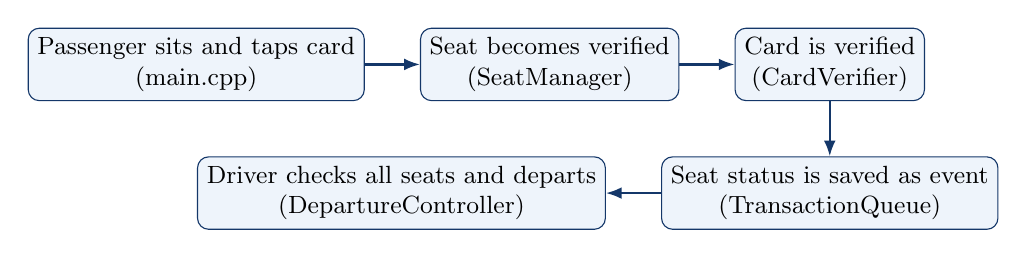
\begin{tikzpicture}[
node distance=7mm,
box/.style={
rectangle,
rounded corners,
draw=GEUBlue,
fill=GEULightBlue,
minimum width=2.10cm,
minimum height=9mm,
align=center,
font=\small
},
arrow/.style={
-{Latex[length=2mm]},
thick,
draw=GEUBlue
}
]

\node[box] (a) {Passenger sits and taps card\\(main.cpp)};
\node[box,right=of a] (b) {Seat becomes verified\\(SeatManager)};
\node[box,right=of b] (c) {Card is verified\\(CardVerifier)};
\node[box,below=of c] (d) {Seat status is saved as event\\(TransactionQueue)};
\node[box,left=of d] (e) {Driver checks all seats and departs\\(DepartureController)};

\draw[arrow] (a)--(b);
\draw[arrow] (b)--(c);
\draw[arrow] (c)--(d);
\draw[arrow] (d)--(e);

\end{tikzpicture}

\end{center}

% \vspace{4mm}

\begin{columns}[T,totalwidth=\textwidth]

\column{.52\textwidth}

\textbf{\color{GEUBlue}Major Components}

\begin{itemize}\itemsep2pt
\item \placeholder{Seat state module: Seat, SeatManager}
\item \placeholder{Fare module: Payment, CardPayment, CardVerifier}
\item \placeholder{Event log and departure: TransactionQueue, DepartureController}
\end{itemize}

\column{.52\textwidth}

\textbf{\color{GEUBlue}Changes Since Phase-I}

\begin{itemize}\itemsep2pt
\item \placeholder{Single-system design, no network protocol}
\item \placeholder{New event queue that records every seat event}
\item \placeholder{Departure rule: no unverified seat allowed}
\end{itemize}

\end{columns}

\vfill

% \smallnote{ Brief Discussion: Present the updated architecture and explain how individual modules communicate with each other. }

\end{frame}

% ============================================================
% SLIDE 6
% ============================================================
\begin{frame}{Module Design \& Functional Requirements}

\vspace{-8mm}

\begin{columns}[T,totalwidth=\textwidth]

\column{.48\textwidth}

\textbf{\color{GEUBlue}Major Modules}

\begin{enumerate}\itemsep3pt
\item \placeholder{Seat State \& Updation (Seat, SeatManager)}
\item \placeholder{Fare \& Card Verification (Payment, CardPayment, CardVerifier)}
\item \placeholder{Event Queue (Passenger, Transaction, TransactionQueue)}
\item \placeholder{Status Panel \& Departure (DriverControl, DepartureController)}
\end{enumerate}

\column{.48\textwidth}

\textbf{\color{GEUBlue}Functional Requirements}

\begin{itemize}\itemsep3pt
\item \placeholder{Mark a seat Empty, Occupied Unverified or Occupied Verified}
\item \placeholder{Verify fare on a valid card tap and reject invalid cards}
\item \placeholder{Log every seat and verification event}
\item \placeholder{Show the seat map and block departure while any seat is unverified}
\end{itemize}

\end{columns}

\vfill

\begin{block}{Module Dependency}
\placeholder{
main.cpp calls SeatManager, CardVerifier updates seat state, event goes to TransactionQueue, DepartureControl reads seat state to decide rediness.
}
\end{block}

% \smallnote{ Brief Discussion: Explain what each module does and how it contributes to the complete system. }

\end{frame}

% ============================================================
% SLIDE 7
% ============================================================
\begin{frame}{Technology Stack \& Development Methodology}

\begin{columns}[T,totalwidth=\textwidth]

\column{.48\textwidth}

\begin{block}{Technology Stack}

\begin{itemize}\itemsep2pt
\item Programming: \placeholder{C++ 17}
% \item Database: \placeholder{MySQL / PostgreSQL}
\item Framework: \placeholder{C++ STL}
\item Development Tool: \placeholder{VS Code, g++}
\item Version Control: \placeholder{Git / GitHub}
\end{itemize}

\end{block}

\column{.48\textwidth}

\begin{block}{Development Methodology}

\begin{enumerate}\itemsep2pt
\item Requirement Analysis
\item System Design
\item Module Development
\item Integration
\item Testing \& Validation
\end{enumerate}

\end{block}

\end{columns}

\vfill

% \smallnote{ Brief Discussion: Explain why the selected technologies are appropriate and how the team is following the development methodology. }

\end{frame}

% ============================================================
% SLIDE 8
% ============================================================
\begin{frame}{Implementation of PBL Course Concepts}

\scriptsize

\begin{center}

\renewcommand{\arraystretch}{1.25}

\begin{tabularx}{.96\textwidth}
{@{}>{\bfseries}p{3.0cm}X p{2.5cm}@{}}

\toprule
Course & Concepts Actually Implemented & Project Module\\
\midrule

Data Structures in C &
\placeholder{Arrays (seat storage), Linked Lists, Queues (event log)} &
\placeholder{Seat, SeatMangager, TransactionQueue}\\

\midrule

OOPs with C++ &
\placeholder{Classes and objects, encapsulation, inheritance (Payment → CardPayment), STL} &
\placeholder{Seat, Payment, CardPayment, CardVerifier}\\


% Operating Systems &
% \placeholder{Processes, Scheduling, Memory, IPC, Synchronization, etc.} &
% \placeholder{Module X}\\

% DBMS &
% \placeholder{SQL, Transactions, Normalization, Indexing, etc.} &
% \placeholder{Module Y}\\

\bottomrule

\end{tabularx}

\end{center}

\vfill

% \begin{center}
% \colorbox{GEULightBlue}{
% \parbox{.88\textwidth}{
% \centering
% \textbf{Important:}
% Mention only those concepts that have been
% \textbf{actually implemented} in the project.
% }}
% \end{center}

% \smallnote{
% Brief Discussion: Students should explain where and how each course
% concept is technically implemented.
% }

\end{frame}

% ============================================================
% SLIDE 9
% ============================================================
\begin{frame}{Development \& Implementation Progress}

\scriptsize
\vspace{-8mm}

\begin{center}

\renewcommand{\arraystretch}{1.25}

\begin{tabularx}{.96\textwidth}
{@{}p{3cm}p{2.2cm}X@{}}

\toprule
\textbf{Module} &
\textbf{Status} &
\textbf{Work Completed}\\
\midrule

\placeholder{Seat State (Seat, SeatManager)} &
Completed &
\placeholder{Three seat states implemented; interfaces being finalized for integration}\\

\placeholder{Fare Verification (Payment, CardPayment, CardVerifier)} &
In Progress &
\placeholder{A card tap marks the seat Verified; partially integrated, logic being completed}\\

\placeholder{Event Queue (Passenger, Transaction, TransactionQueue)} &
In Progress &
\placeholder{Implemented; records every seat and verification event}\\

\placeholder{Driver Panel \& Departure (DriverControl, DepartureController)} &
Completed &
\placeholder{Departure rule tested (bus waits while any seat is unverified)}\\

\placeholder{Database \& Interface} &
Pending &
\placeholder{planned}\\

\bottomrule

\end{tabularx}

\end{center}

\vspace{-3mm}

\begin{center}
\colorbox{GEULightBlue}{
\parbox{.65\textwidth}{
\centering
\textbf{Overall Project Completion:}
\placeholder{Approximately 75\%}
}}
\end{center}

\vfill

% \smallnote{ Brief Discussion: Clearly differentiate between completed, in-progress and pending development. Do not present proposed work as completed work. }

\end{frame}

% ============================================================
% SLIDE 10
% ============================================================
\begin{frame}{Working Prototype / Demonstration}

\begin{columns}[T,totalwidth=\textwidth]

\column{.45\textwidth}

\textbf{\color{GEUBlue}Implemented Features}

\begin{itemize}\itemsep3pt
\item \placeholder{Menu-driven console application (main.cpp)}
\item \placeholder{Seat states: Empty, Occupied Unverified, Occupied Verified}
\item \placeholder{Event log of every seat and verification event}
\item \placeholder{Departure blocked while any seat is unverified}
\end{itemize}

\column{.51\textwidth}

\begin{block}{Prototype / Output}

\centering

\placeholder{
    \includegraphics[width=60mm\textwidth]{image.png}
}

\end{block}

\end{columns}

\vfill

% \smallnote{ Brief Discussion: Demonstrate the actual working implementation. Students should preferably provide a live demonstration in addition to screenshots wherever applicable. }

\end{frame}

% ============================================================
% SLIDE 11
% ============================================================
\begin{frame}{Testing, Results \& Validation}

\scriptsize

\begin{center}

\renewcommand{\arraystretch}{1.3}

\begin{tabularx}{.96\textwidth}
{@{}p{2.1cm}X X p{1.4cm}@{}}

\toprule
Test / Module &
Expected Result &
Observed Result &
Status\\
\midrule

\placeholder{Compilation test (g++, C++17)} &
\placeholder{Code compiles without errors} &
\placeholder{Compiles fine} &
Pass\\

\placeholder{Seat state and departure logic} &
\placeholder{Bus does not leave while any seat is red; clears when all are verified} &
\placeholder{Departure blocked until every seat is verified} &
Pass\\

\placeholder{Full team integration test} &
\placeholder{All modules merged and run through main.cpp} &
\placeholder{merged successfully} &
\placeholder{Pass}\\

\bottomrule

\end{tabularx}

\end{center}

\vspace{3mm}

\begin{block}{Results / Validation}
\placeholder{
All tests passed successfully with no compilation or runtime errors.
}
\end{block}

% \smallnote{ Brief Discussion: Results should be supported by actual testing or experimental evidence rather than assumptions. }

\end{frame}

% ============================================================
% SLIDE 12
% ============================================================
\begin{frame}{GitHub Repository \& Development Activity}

\begin{columns}[T,totalwidth=\textwidth]

\column{.46\textwidth}

\textbf{\color{GEUBlue}Repository Information}

\begin{itemize}\itemsep3pt
\item GitHub Link: \placeholder{github.com/kjj2608/TapNGo}
\item README.md: \placeholder{Updated}
\item Contributors: \placeholder{All Members Added}
\item Repository Status: \placeholder{Updated}
\item Branches: \placeholder{local branches for each member}
\end{itemize}

\column{.50\textwidth}

\textbf{\color{GEUBlue}Development Activity}

\begin{itemize}\itemsep3pt
\item \placeholder{Repository created with branches for each member}
\item \placeholder{source code updated regularly}
\item \placeholder{Individual contribution are visible}
\item \placeholder{Latest implementation uploaded of working prototype}
\item \placeholder{Documentation maintained}
\end{itemize}

\end{columns}

\vfill

% \begin{center}
% \colorbox{GEULightBlue}{
% \parbox{.88\textwidth}{
% \centering
% \textbf{Requirement:}
% All team members must be contributors and must
% \textbf{commit individually using their own GitHub accounts}.
% }}
% \end{center}

% \smallnote{
% Brief Discussion: Show repository activity, README, contributor list
% and commit history during the presentation.
% }

\end{frame}

% ============================================================
% SLIDE 13
% ============================================================
\begin{frame}{Individual Contribution}

\scriptsize

\begin{center}

\renewcommand{\arraystretch}{1.35}

\begin{tabularx}{.96\textwidth}
{@{}p{2.0cm}p{2.0cm}X p{1.6cm}@{}}

\toprule
Member &
Role &
Technical Contribution &
GitHub Commits\\
\midrule

\placeholder{Karnika Jain} &
\placeholder{Team Lead and Seat verification} &
\placeholder{Seat management classes, seat state logic and OOP architecture} &
\placeholder{9}\\

\placeholder{Anirudh Bahuguna} &
\placeholder{main and Payment Verification} &
\placeholder{Card Verifier; connecting fare verification to seat state updates} &
\placeholder{14}\\

\placeholder{Aparajita Pant} &
\placeholder{Departure and Panel} &
\placeholder{Departure readiness logic, driver status panel and module integration} &
\placeholder{13}\\

\placeholder{Aaditya Budakoti} &
\placeholder{Transation Queue and testing} &
\placeholder{mainting the records of all payments and testing} &
\placeholder{2}\\

\bottomrule

\end{tabularx}

\end{center}

\vspace{3mm}

% \begin{block}{Individual Evaluation}
% Every member should be prepared to explain and demonstrate
% their own technical contribution to the project.
% \end{block}

% \smallnote{
% Brief Discussion: Contributions should be specific and verifiable.
% Avoid generic statements such as ``helped in coding'' or
% ``worked on documentation''.
% }

\end{frame}

% ============================================================
% SLIDE 14
% ============================================================
\begin{frame}{Challenges, Remaining Work \& Phase-III Roadmap}

\vspace{-7mm}

\begin{columns}[T,totalwidth=\textwidth]

\column{.52\textwidth}

\textbf{\color{GEUBlue}Challenges Faced}

\begin{itemize}\itemsep2pt
\item \placeholder{Developing separate C++ modules and keeping their interfaces compatible}
\item \placeholder{Keeping seat states consistent during occupancy and fare verification}
\item \placeholder{Errors when integrating the seat, card and driver panel modules}
\end{itemize}

\vspace{2mm}

\textbf{\color{GEUBlue}Solutions / Learning}

\begin{itemize}\itemsep2pt
\item \placeholder{Each module tested on its own before integration}
\item \placeholder{Work divided by member; Git/GitHub branches}
\end{itemize}

\column{.48\textwidth}

\textbf{\color{GEUBlue}Phase-III Roadmap}

\begin{enumerate}\itemsep3pt
\item \placeholder{Inclusion of a Database to maintain records and fares}
\item \placeholder{Finish Payment and card verification modules}
\item \placeholder{Improve the User Interface}
\item \placeholder{Stop selection}
\item \placeholder{Testing / optimization}
\end{enumerate}

\end{columns}

\vfill

% \smallnote{
% Brief Discussion: Explain genuine technical challenges and provide
% a realistic roadmap for completing the project before Phase-III.
% }

\end{frame}

% ============================================================
% SLIDE 15
% ============================================================
\begin{frame}{Expected Outcomes \& References}

\begin{columns}[T,totalwidth=\textwidth]

\column{.47\textwidth}

\textbf{\color{GEUBlue}Expected Final Outcomes}

\begin{itemize}\itemsep3pt
\item \placeholder{Working menu-driven C++ prototype of TapNGo}
\item \placeholder{Grey / red / green driver seat map}
\item \placeholder{Reduced boarding delay from manual fare checks}
\item \placeholder{Automatic departure decision: no unverified seat}
\item \placeholder{Can later be extended with real card readers}
\end{itemize}

\column{.47\textwidth}

\textbf{\color{GEUBlue}References}

\begin{enumerate}\itemsep3pt
\item \placeholder{cppreference.com– C++17 and STL documentation}
\item \placeholder{Git documentation, git-scm.com/doc}
\item \placeholder{Project repository: github.com/kjj2608/TapNGo}
\end{enumerate}

\vfill

\begin{center}

\colorbox{GEUBlue}{
\parbox{.78\textwidth}{
\centering
\color{white}
\textbf{Thank You}\\
Questions \& Suggestions
}}

\end{center}

\end{columns}

\vfill

% \smallnote{
% Brief Discussion: Conclude with the tangible final outcome expected
% from the project and cite the major technical/research resources used.
% }

\end{frame}

\end{document}
